% --------------------------------------
% labels: \label{mil2:res:[type]:[name]}
% --------------------------------------
% PAST TENSE

The free electron fraction as computed from the Saha and Peebles equations in their respective regimes is plotted in \cref{mil2:res:fig:electron_fraction}.
\begin{figure}[!ht]
    \centering
    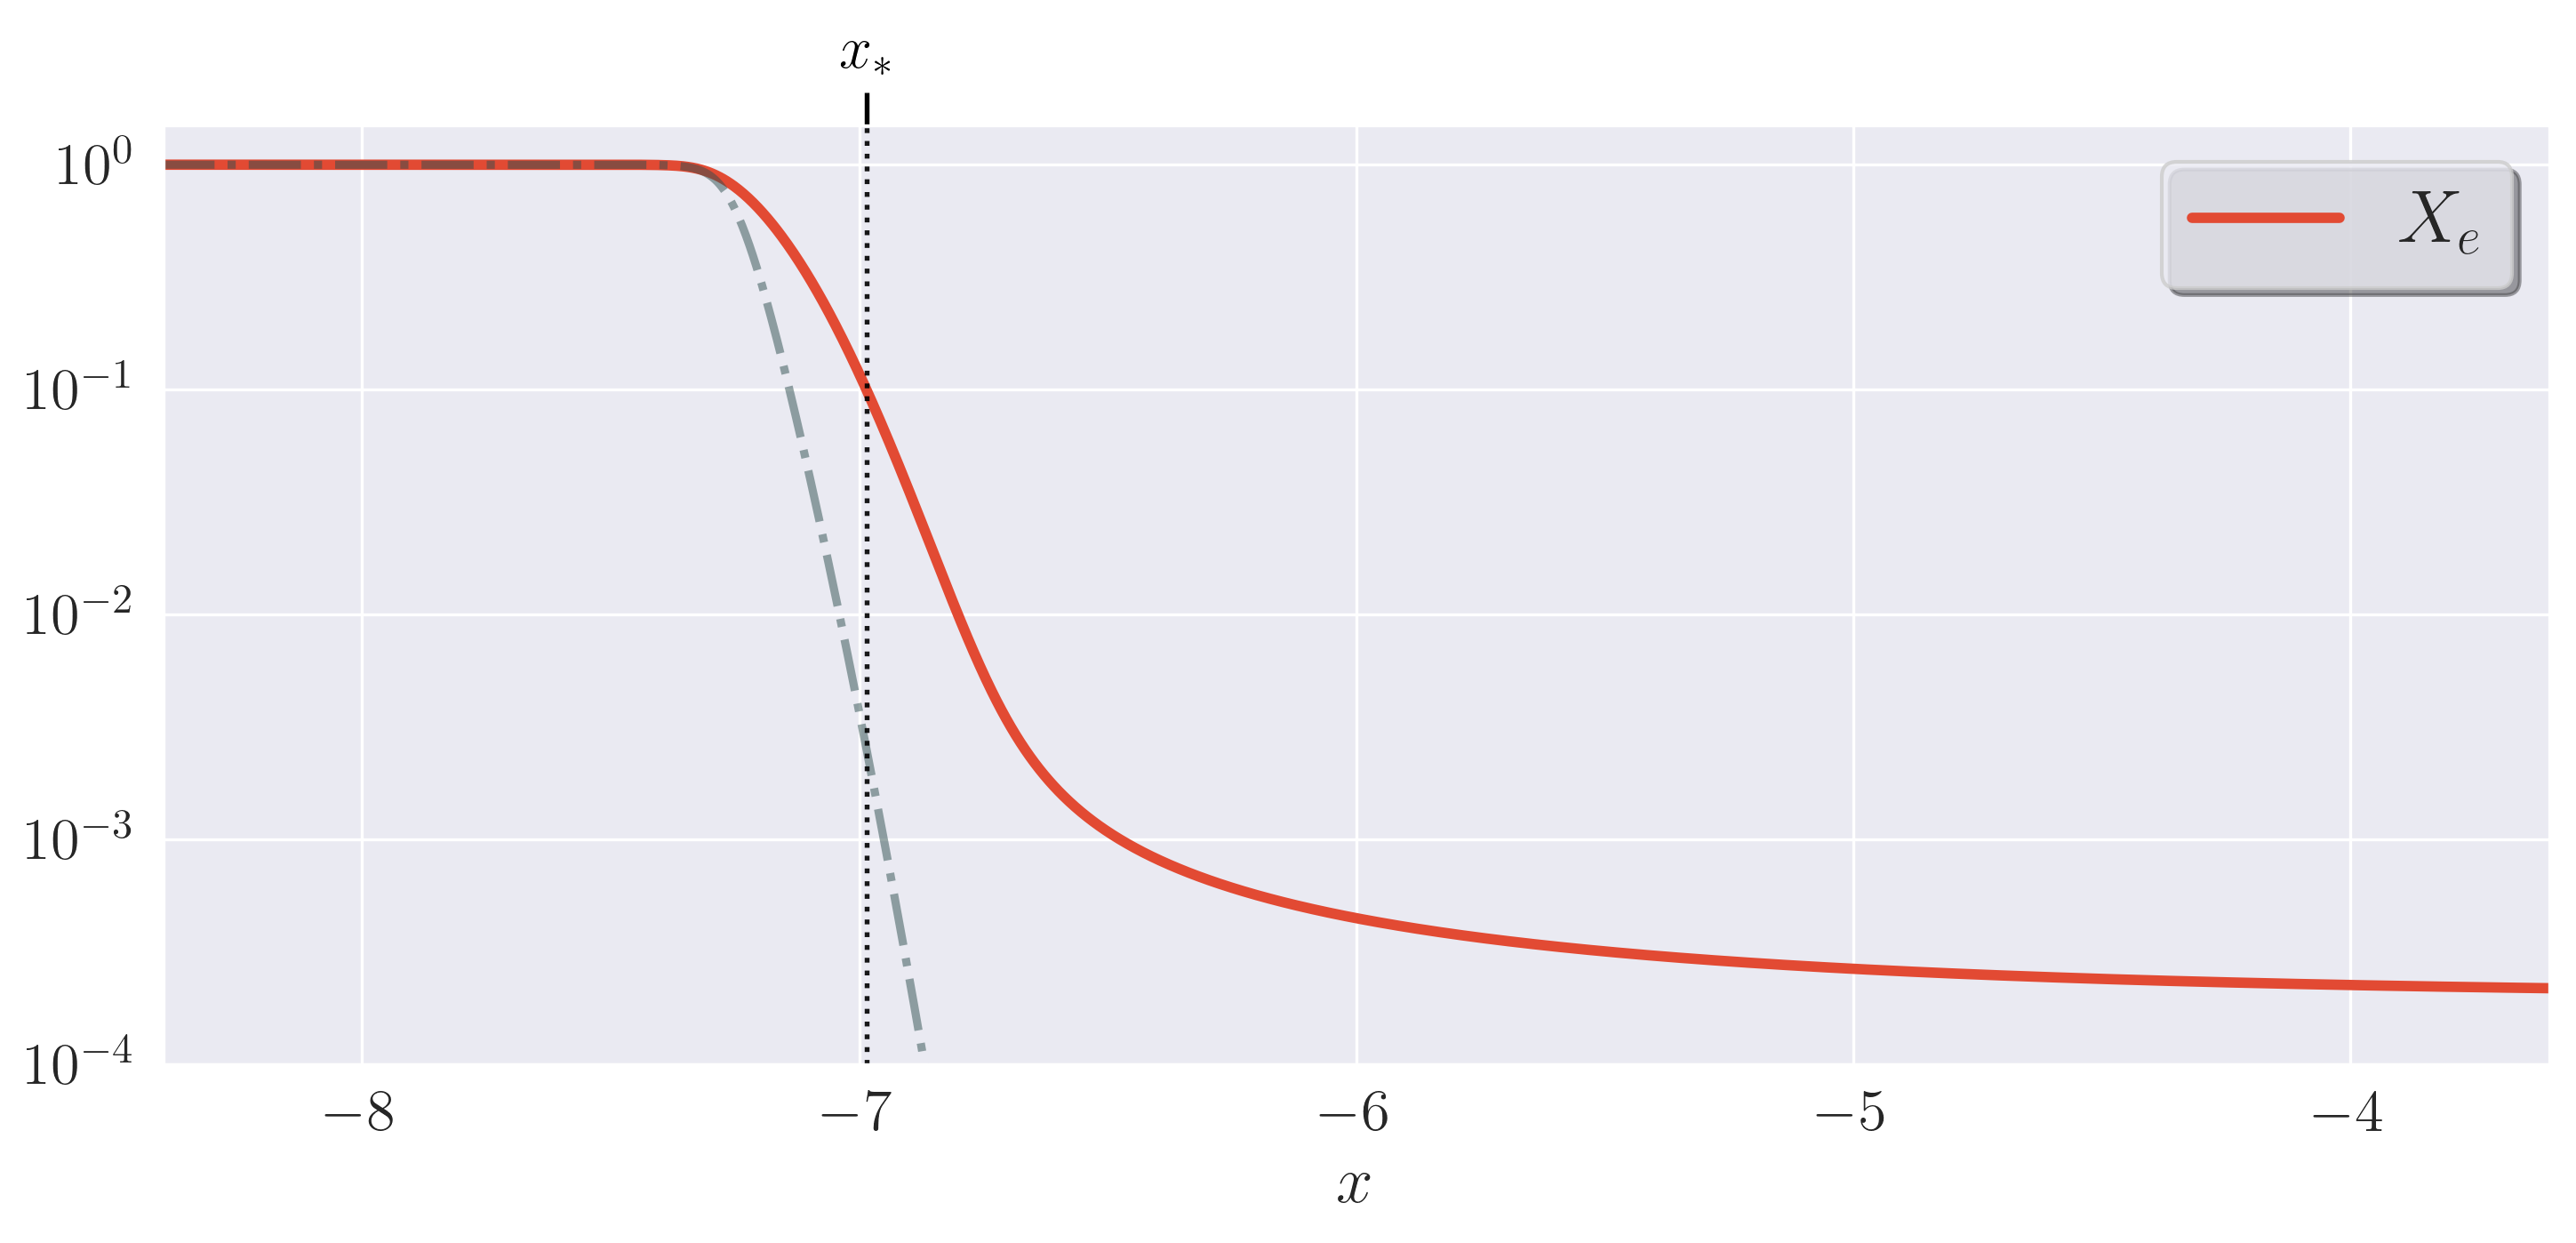
\includegraphics[width=\linewidth]{milestone2/electron_fraction.png} 
    \caption{\textcolor{blue}{The fractional electron density $X_e(x)$ resulting from the Peebles and Saha equations.}} 
    \label[fig]{mil2:res:fig:electron_fraction}
\end{figure}
As elaborated in \cref{mil2:imp:sec:tau_gt} we calculated the optical depth and visibility function and their derivatives.
We present the optical depth and its derivatives in \cref{mil2:res:fig:optical_depth}. The visibility function is demonstrated in \cref{mil2:res:fig:visibility_function} scaled to be comparable to its (also scaled) derivatives.
\begin{figure}[!ht]
    \centering
    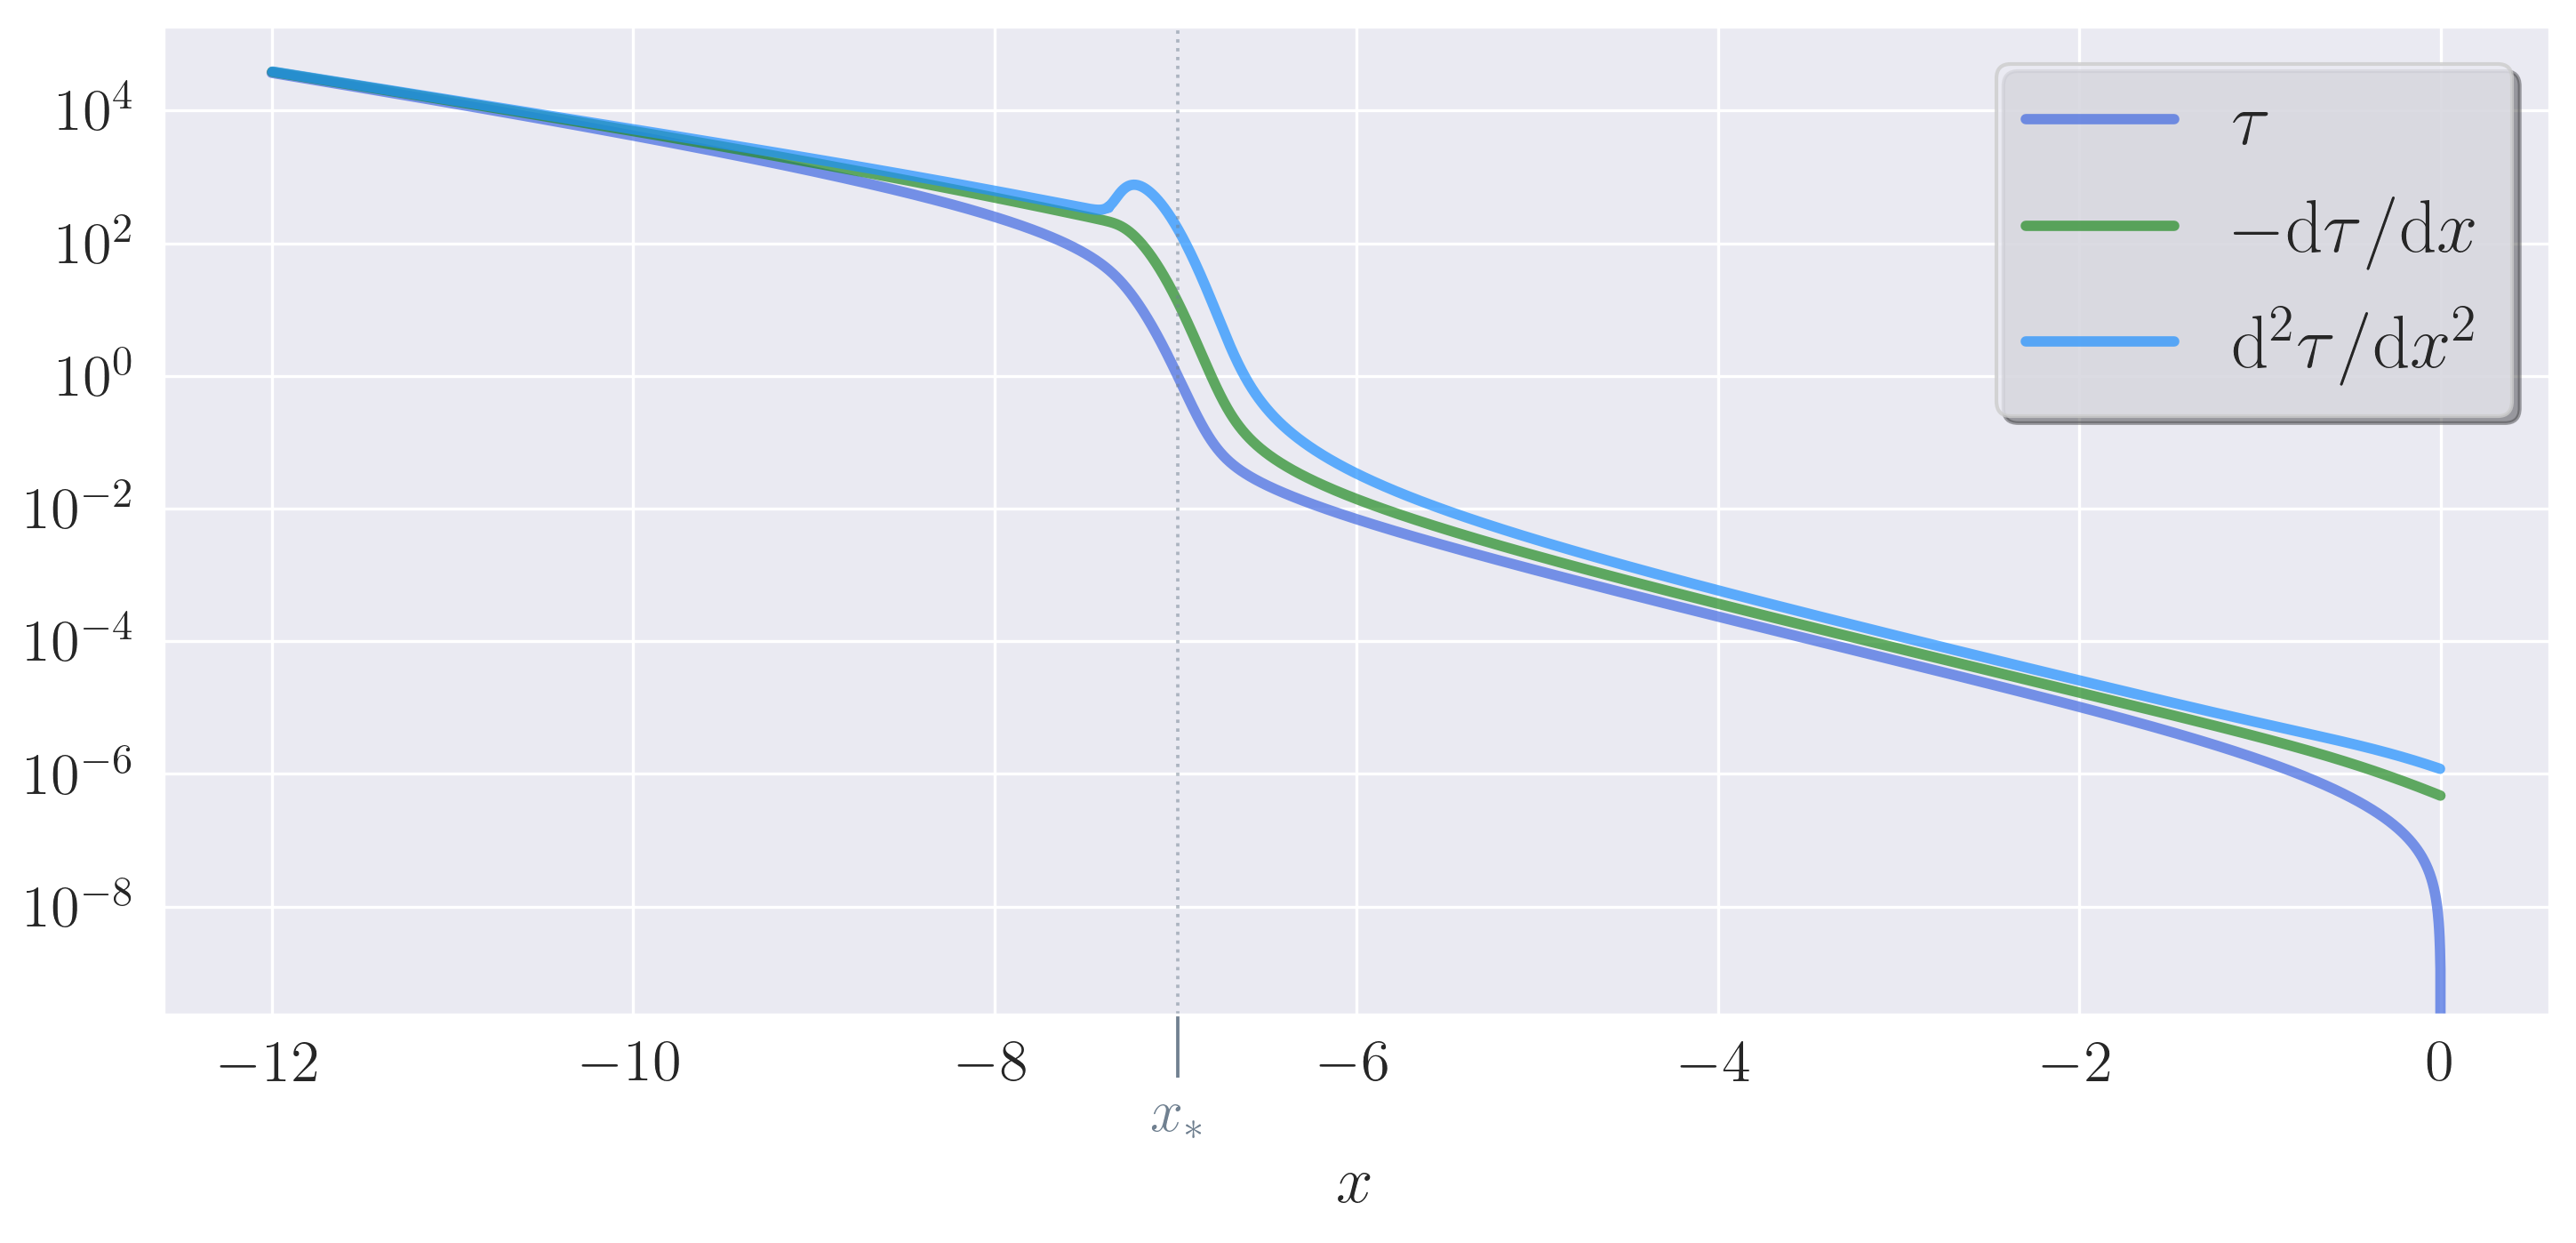
\includegraphics[width=\linewidth]{milestone2/optical_depth_misc.png} 
    \caption{\textcolor{blue}{The optical depth $\tau(x)$ and its derivatives $-\dv{\tau(x)}{x}$ and $\dv[2]{\tau(x)}{x}$ as functions of logarithmic scale factor $x$.}} 
    \label[fig]{mil2:res:fig:optical_depth}
\end{figure}
\begin{figure}[!ht]
    \centering
    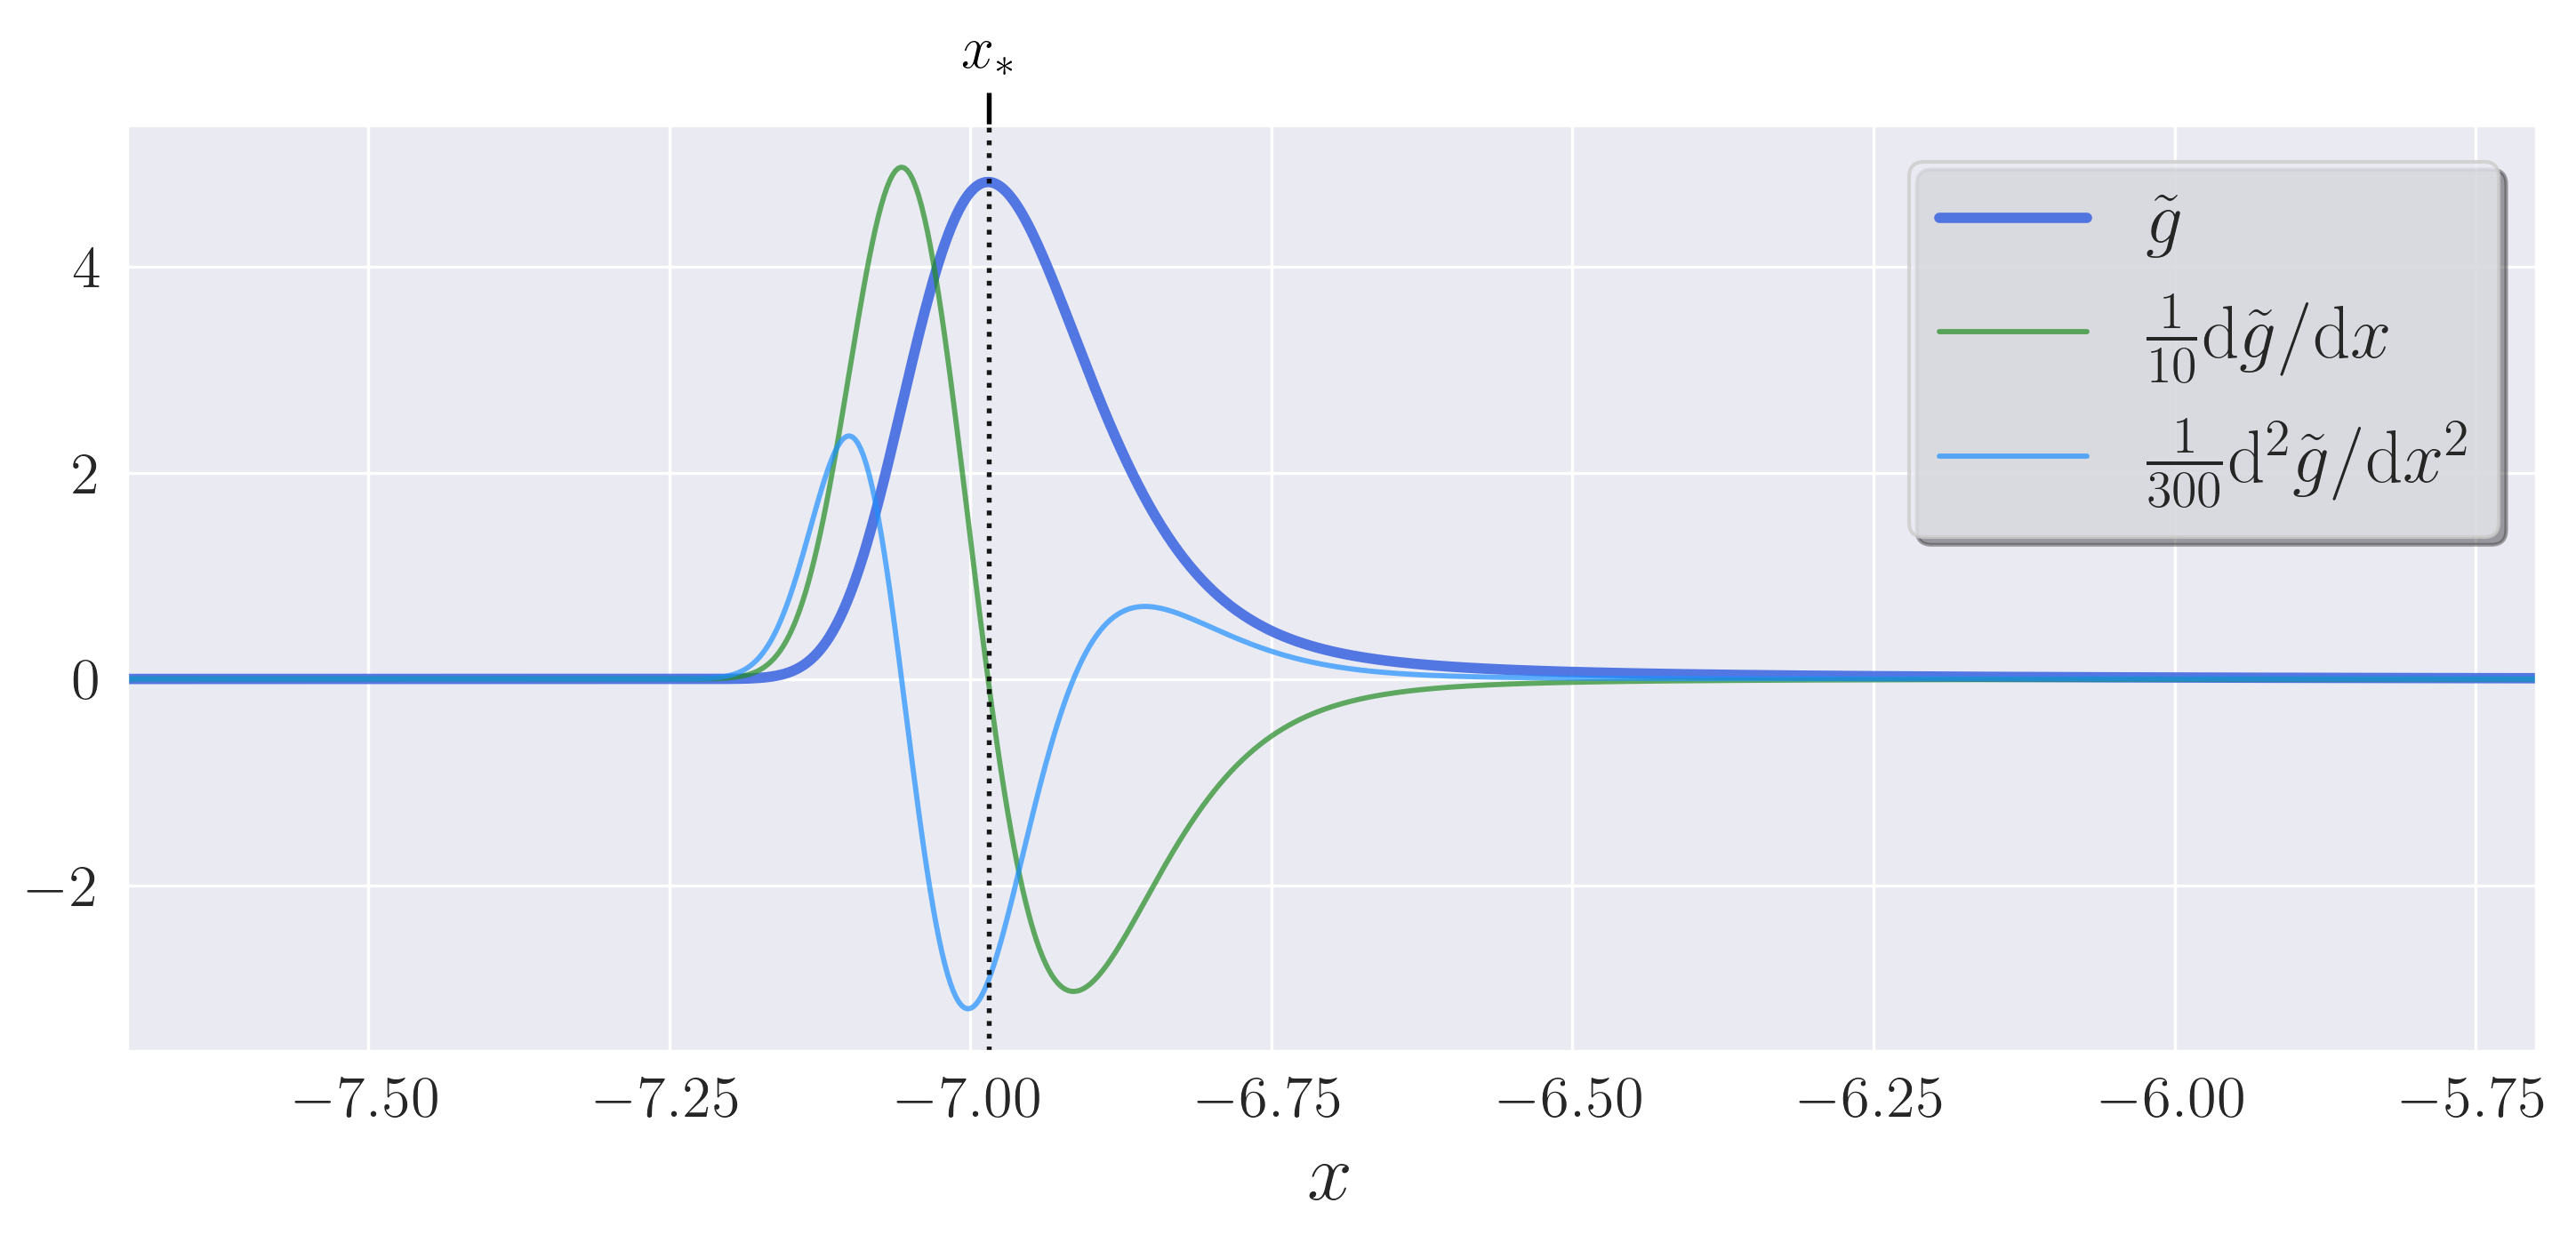
\includegraphics[width=\linewidth]{milestone2/visibility_function_misc.png} 
    \caption{\textcolor{blue}{The visibility function $\gti(x)$ and its derivatives $\dv{\gti(x)}{x}$ and $\dv[2]{\gti(x)}{x}$ as functions of logarithmic scale factor $x$.}} 
    \label[fig]{mil2:res:fig:visibility_function}
\end{figure}

Using our definitions of the time of last scattering surface and recombination from \cref{mil2:theo:sec:optical_depth} and \cref{mil2:theo:sec:recombination}, we measured the logarithmic scale factor, redshift and cosmic time at these events. We present the results in \cref{mil2:res:tab:time_of_events} in addition to today's value of the freece-out (FO) electron abundance and the sound horizon at decoupling. The number of signifant figures is exaggerated to point out the small differences.

\begin{table}[h]
    \setlength\tabcolsep{0pt}
    \caption{The values of the logarithmic scale factor $x$, the redshift $z$ and the cosmic time $t$ corresponding to two events in the history of the universe.}
    \label[tab]{mil2:res:tab:time_of_events}
    \begin{tabular*}{\linewidth}{@{\extracolsep{\fill}} l *{1}{d{2.4}} *{1}{d{4.1}} *{1}{d{3.5}}}
        \toprule
        & \multicolumn{1}{c}{$x$} & \multicolumn{1}{c}{$z$} & \multicolumn{1}{c}{$t$} \\
        \midrule
        Recombination           & -6.9853 & 1079.7 & 377.95\unit{ka} \\
        Last scattering surface & -6.9854 & 1079.8 & 378.04\unit{ka} \\
        \midrule
        \multicolumn{2}{l}{FO free electron abundance today: }& \multicolumn{2}{c}{$X_{e0} = 2.0261\cross10^{-4}$}\\
        \multicolumn{2}{l}{Sound horizon at decoupling: }& \multicolumn{2}{c}{$r_s(x_*) = 145.30\unit{Mpc}$}\\
        \bottomrule
    \end{tabular*}
\end{table}